\def\be{\begin{equation}}
\def\ee{\end{equation}}
\pdfpageattr {/Group << /S /Transparency /I true /CS /DeviceRGB>>}
\newcommand{\nucl}[3]{ \ensuremath{ \phantom{\ensuremath{^{1}_{#2}}} \llap{\ensuremath{^{#1}}} \llap{\ensuremath{_{\rule{0pt}{.75em}#2}}} \mbox{#3} } }





\documentclass[12pt]{article}
\usepackage{graphicx}
\usepackage{notoccite}
\usepackage{epigraph} % epigraph
\usepackage{float}
\usepackage[hyphens]{url}
\usepackage[square, numbers, comma, sort&compress]{natbib}  % Use the "Natbib" style for the references in the Bibliography
\usepackage{verbatim,listings}  % Needed for the "comment" environment to make LaTeX comments
\usepackage{array}  % Needed for the "comment" environment to make LaTeX comments
\usepackage{vector}  % Allows "\bvec{}" and "\buvec{}" for "blackboard" style bold vectors in maths

% \documentclass[a4paper,12pt]{article}
%\usepackage[a4paper,vmargin={20mm,20mm},hmargin={20mm,20mm}]{geometry}
\usepackage{amsmath,amsfonts,amsthm,color,psfrag,epsf,graphicx}
% \usepackage{pstricks}
\usepackage{enumerate,caption}
%\usepackage[lined,algonl,boxed]{algorithm2e}
\usepackage[ruled,linesnumbered,vlined]{algorithm2e}
\usepackage{float}
% \SpecialCoor
\def\subsum{\mathit{\Sigma}}




\def\ifthesis{\iftrue}
\setcounter{secnumdepth}{2}
\newenvironment{myindentpar}[1]%
{\begin{list}{}%
		{\setlength{\leftmargin}{#1}}%
		\item[]%
	}
	{\end{list}}




\graphicspath{{Figures/}}  % Location of the graphics files (set up for graphics to be in PDF format)
\usepackage{epigraph} % epigraph
%customize: \setlength{\epigraphwidth}{7cm}\setlength{\epigraphrule}{0pt}
%use: \epigraph{text}{reference}

%customize: \setlength{\epigraphwidth}{7cm}\setlength{\epigraphrule}{0pt}
%use: \epigraph{text}{reference}
\begin{document}
\bibliographystyle{unsrt}
\section*{Declaration}
Figures 4, 6, 7, 9, 10 and the accompanying discussion have previously been published in \cite{me}. 
\section{Introduction}
The ball-pen probe is an advanced probe technique designed to directly measure the plasma potential ($\Phi$). As discussed in Chapter 2, a Langmuir probe inserted into a plasma floats not at the plasma potential, but at a floating potential $(V_f)$ which is negative with respect to the plasma potential.  
The theory of Langmuir probes allows the value of the plasma potential to be determined from the current (I) - voltage (V) curve of a Langmuir probe. Assuming the probe operates in the thin sheath limit, a simple expression \cite{bound2} relates the floating potential of the probe ($V_{LP}$) to the local plasma potential
\begin{equation}
V_{LP} = \Phi - T_e\ln(R)
\label{eq:ideal}
\end{equation}
where $T_e$ is the electron temperature in eV and R the ratio of the electron saturation current ($I^-_{sat}$) divided by the ion saturation current ($I^+_{sat}$). The logarithm of $R$ is often denoted as $\alpha$ such that 
\begin{equation}
\alpha_{LP} = \ln(R) = \ln\left(\frac{I^-_{sat}}{I^+_{sat}}\right)
\end{equation}
In principle it is possible to sweep the bias voltage applied to a Langmuir probe to derive $V_{LP}$, $T_e$ and $\alpha_{LP}$. The local plasma potential can then be obtained from equation \ref{eq:ideal}. However, in practice, especially in fusion plasmas,  it is not possible to measure $R$. In these plasmas, probes operate in a restricted region of the I - V curve from floating to ion saturation. This allows measurements of $n_e$ and $T_e$ to be made whilst avoiding damage to the probe and the problem of spuriously high $T_e$ measurements  \cite{JET_TE}, \cite{matthews}, \cite{iv_safe_region}, \cite{pin-plate-pitts}.

Measurements of the plasma potential ($\Phi$) and its fluctuations are vital for modelling transport phenomena in the edge region of tokamaks \cite{Adamek2009}. Turbulent structures (filaments) in the scrape-off layer are electrostatic and are advected towards the first-wall by E x B drifts arising from plasma potential fluctuations across the filament cross-section \cite{filaments}. The strength and spatial scale of these potential fluctuations can be predicted, however robust measurements of such fluctuations are lacking, making it difficult to fully validate models of radial transport in the SOL \cite{blobs}. Various advanced probe techniques have been developed that aim to measure the plasma potential directly without needing an electron temperature measurement. These include emissive probes \cite{emissive} which will be discussed in Chapter X and the Ball-Pen Probe (BPP) \cite{BPP}. The emissive probe is not well suited to fusion plasmas as it requires a thin filament of wire to be exposed to the plasma making it structurally weak as opposed to the BPP which is a robust diagnostic capable of surviving high heat loads \cite{NW}. The BPP was designed to reduce the ratio of saturation currents to unity so that the probe would float at the plasma potential, as evident from equation \ref{eq:ideal}. With a typical filament size on the order of a cm and velocities on the order of km/s, microsecond time resolution is required to track the evolution of the potential between and during filament events \cite{filament_res}. The potential capability of the BPP to measure the plasma potential using a DC, floating measurement allows sufficient time resolution to measure these potential fluctuations \cite{BPP_resolution}. Despite empirical confirmation of the BPPs capabilities \cite{Adamek2009}, \cite{BPP},\cite{BPP-COMPASS}, \cite{BPP-MAST}, \cite{low_temp} the probe is lacking a model based on first principles to confirm the collection mechanism. Presented in this chapter, are the results of three dimensional PIC simulations to explore the behaviour of the BPP.


%with an overview of the importance of accurate, highly resolved plasma potential measurements.
This chapter begins by describing the principles behind the design of the BPP, an overview of the empirical evidence for the workings of the BPP are then given. The PIC simulation model is then described and results obtained from it are discussed in the remainder of the chapter. Simulations are used to investigate, the collection mechanism of the BPP as well as the capability of the BPP to measure the plasma potential and the electron temperature. The chapter finishes with future work and concluding remarks. 

\section{The Ball-Pen Probe Design and Theory}
There are currently two designs for the BPP. The initial design \cite{BPP} consisted of a conically shaped collector shielded by a tube of insulating boron nitride. This design is shown in figure \ref{fig:BPP_Adamek}. The latter design is equipped with  a flat, rather than conical collector and will be discussed later in this section.
\begin{figure}[H]
\centering
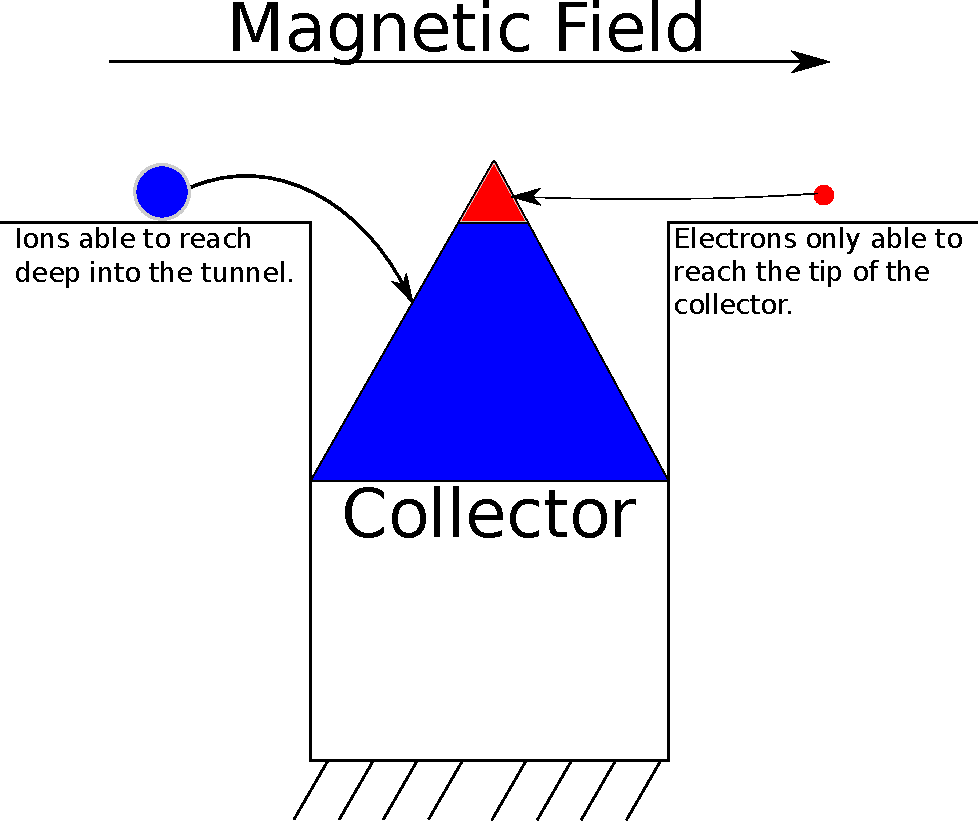
\includegraphics[height=10cm]{adamek_probe.pdf}
\caption{A schematic of the initial design of the BPP proposed by Adamek \cite{BPP}. The probe is orientated such that the axis of the tunnel is perpendicular to the magnetic field.}
\label{fig:BPP_Adamek}
\end{figure}
The probe is aligned such that the axis of the tunnel is near perpendicular to the magnetic field. The vertical position of the collector can be adjusted to alter the collection area that is exposed to the plasma. By recessing the collector inside the tunnel, the BPP aims to exploit the difference between the ion Larmor radius ($\rho_i$) and the electron Larmor radius ($\rho_e$) to achieve a value of $R=1$. As shown in figure \ref{fig:BPP_Adamek}, electrons with their small gyro-orbits will only be able to access the small tip of the collector, with area ($A_e$), whereas the larger ion gyro-orbit allows them to enter deep into the tunnel and access a much larger collection area ($A_i$). The electrons have a much higher parallel current density ($J_e$) relative to that of the ions ($J_i$) and so a larger ion collection area is required to equalise the saturation currents to the collector. In order for the ion saturation current to equal the electron saturation current, the following criteria must be met 
\begin{equation}
I_e = A_e J_E \hspace{0.25cm}= \hspace{0.25cm} I_i = A_i J_i
\end{equation}
As $J_e > J_i$ it is only possible to achieve a value of $R=1$ if $A_e < A_i$.  By adjusting the effective collection areas of the probe for the different species it was envisaged that an optimum recession depth would be found for which $R=1$ \cite{BPP}. In the ideal case, it was thought that recessing the probe further than this height would result in a larger ion saturation current than electron saturation current, leading to a value of $R<1$ and a floating potential that was positive with respect to the plasma potential. Likewise, raising the probe above this optimum depth would lead to values of $R>1$ as seen for a typical probe, in which case the probe collector would float negatively with respect to the plasma potential.

This simple model, first proposed by Adamek, shows some qualitative agreement with experimental data, but there are empirical features which can not be explained by this model, suggesting there is more complex physics to be considered. These empirical features will be discussed below. In addition, in \cite{BPP_flat}, an alternative BPP design with a flat, cylindrical collector was implemented and results compared favourably with the initial BPP conical design, demonstrating that the conical collector is not essential to the BPP collection mechanism.

 It is possible to use a BPP in conjunction with a standard Langmuir probe to make fast measurements of the electron temperature. This has been carried out on multiple tokamak experiments and yielded excellent agreement with Thomson scattering data \cite{BPP_TE}, \cite{BPP-MAST}, \cite{ISTTOK_te}.

The floating potential as measured by a BPP and Langmuir probe (LP) can be written as 
\begin{equation}
V_{BPP} = \Phi - \alpha_{BPP} T_e
\end{equation}
\begin{equation}
V_{LP} = \Phi - \alpha_{LP} T_e
\end{equation}
 

By rearranging these expressions we obtain
\begin{equation}
T_e = \frac{V_{BPP}-V_{LP}}{\alpha_{LP}-\alpha_{BPP}}
\end{equation}
It is not possible to measure $\alpha_{LP}$ in most tokamak experiments as the probe drains too high a current in electron collection mode, however a theoretical value, for a planar Langmuir probe, is given by Stangeby \cite{stangeby-2000}
  
\begin{equation}
\alpha = - \frac{1}{2} \ln \left(2\pi\frac{m_e}{m_i}\left(1+ \frac{T_i}{T_e}\right)\right)
\label{eq:Stangeby}
\end{equation}
Which gives for a hydrogen plasma, assuming $T_i = T_e$, $\alpha_{LP} \approx 2.5$.



  $\alpha_{BPP}$ on the other hand can be measured directly in experiments as the currents to the collector are much lower. It is possible to use these two values along with a Langmuir probe and BPP operated in floating mode to determine $T_e$. All that is needed is a floating potential measurement from each probe, which can be made instantaneously, only limited by the speed of the data acquisition system. In fusion plasmas, $T_e$ is typically measured by sweeping a standard Langmuir probe from ion collection to floating potential and then fitting an exponential to the IV curve. This method is slow relative to the BPP-LP method due to the time it takes to sweep the probe voltage. The BPP-LP method then offers better time resolution and potentially more accurate measurements of $T_e$ as it uses a floating potential measurement from the Langmuir probe which is considered to be in the safe region of the IV curve for a probe in magnetised plasma \cite{iv_safe_region}. 


 % As will be detailed in section \ref{Experiment}, both electron and ion currents are measured at the probe even when the collector is recessed beyond an ion Larmor radius. This was not predicted by the initial proposal for the collection mechanism. It has also been observed in experiments that the ratio $R$ falls approximately to unity once the probe is recessed beyond a few $\rho_e$ and does not vary significantly with further recession. These observations imply that particle transport to the probe is more complex and must occur perpendicular to the magnetic field. In \cite{BPP_flat} it was realised that because recession depth beyond a few $\rho_e$ did not affect probe readings, the conical shape of the collector was not necessary. A flat, cylindrical collector was then implemented and results compared favourably with the initial BPP conical design. 

%Such a design was implemented in MAST \cite{NW}, a schematic for which is shown in figure \ref{fig:bpp_mechanism}. The MAST BPP had a radius of 4 mm and a retraction depth of 5 mm. Adamek's conical probe had a radius of 4 mm and was operated with a variable retraction depth up to 2 mm. 



\begin{figure}[H]
\centering
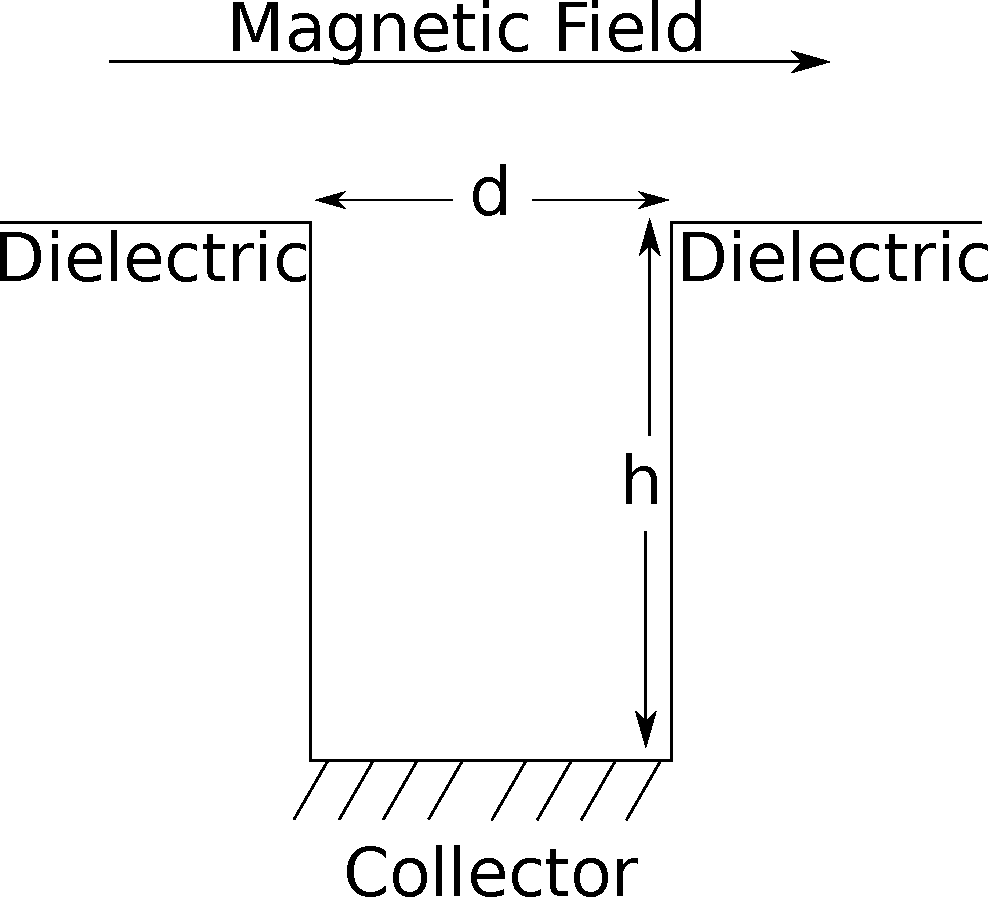
\includegraphics[height=10cm]{flat_collector.pdf}
\caption{A BPP with a flat cylindrical collector. Also referred to as a Katsumata-type probe. $d$ is the diameter of the probe and $h$ the retraction depth.} %The BPP on MAST had a fixed retraction depth of 5 mm and a diameter of 4 mm }
\label{fig:bpp_mechanism}
\end{figure}


%According to the theory once the collector is recessed sufficiently the electron saturation current will be reduced to the extent such that the two saturation currents are equal and so $V_f = V_p$. Increasing the depth beyond this point would lead to $R<1$. However this is contradicted by experimental observations. In experiments it is found that R never quite falls to unity, meaning the electron current to the collector is always greater than the ion current regardless of probe depth. It does however remain close to unity once the probe is recessed sufficiently and the probe floats at the plasma potential. The floating potential remains constant with further recession. These two observations highlight that the collection mechanism is more complicated than the simple theory proposes and that cross-field transport must play a role. 
\section{Empirical Confirmation of the Ball-pen Probe Method}  \label{Experiment} 
BPPs have been used to measure the plasma potential in multiple tokamak experiments including CASTOR\cite{BPP}, COMPASS \cite{BPP-COMPASS}, MAST \cite{BPP-MAST} and ASDEX Upgrade in both L-mode \cite{LandH}, \cite{L-mode} and H-mode \cite{LandH},\cite{Adamek2009}. Comparative measurements of the plasma potential were made using a BPP and a self-emitting Langmuir probe on COMPASS \cite{BPP-SEP} and with a BPP and emissive probe on CASTOR \cite{BPP-EP}. 
BPPs have also been employed in low-temperature, weakly magnetised plasmas \cite{low_temp}, \cite{low_temp2}. In these plasmas the electrons are strongly magnetised but the ions are demagnetised. It was found that the BPP could measure the plasma potential in this case, but the capability of the BPP to shield the electron current was strongly dependent on the probe geometry, only effectively screening the electrons once the radius of the insulating tube was less than the electron Larmor radius \cite{low_temp2}.



Figure \ref{fig:adamek} shows the orginal BPP designed by Adamek alongside experimental results obtained by the probe, taken from \cite{BPP}. In Adamek's initial experiments, an IV curve was produced by sweeping the bias voltage applied to the conical collector, this enabled a value of $R$ to be obtained. As can be seen in figure \ref{fig:adamek}c, the probe behaves as a standard Langmuir probe, with an electron saturation current much greater than the ion saturation current, for positive values of $h$,   where the collector is outside the tunnel and directly exposed to plasma. A large reduction is observed in the electron saturation current, for negative values of $h$, where the collector is recessed inside the probe tunnel, demonstrating the capability of the probe to shield off the electron current. The ion saturation current remains roughly constant for both IV curves which results in a large reduction of $R$ for the recessed collector relative to the exposed collector. The process of sweeping the probe was repeated for various retraction depths, providing a measurement of the floating potential and $\alpha_{BPP}$ as as function of collector depth. This is shown in figure \ref{fig:adamek}d.  As the collector is recessed inside the insulating tube, $\alpha_{BPP}$ approaches zero, although it is never observed to actually reach zero. At a recession depth of $h = -0.5$ mm, corresponding to a recession depth of one ion Larmor radius, $\alpha_{BPP}$ was observed to reach a minimum of $\approx 0.2$ . At this point, if equation \ref{eq:ideal} is valid for the BPP, the collector floats at a potential which should be very close to the plasma potential. 


\begin{figure}[H]
\centering
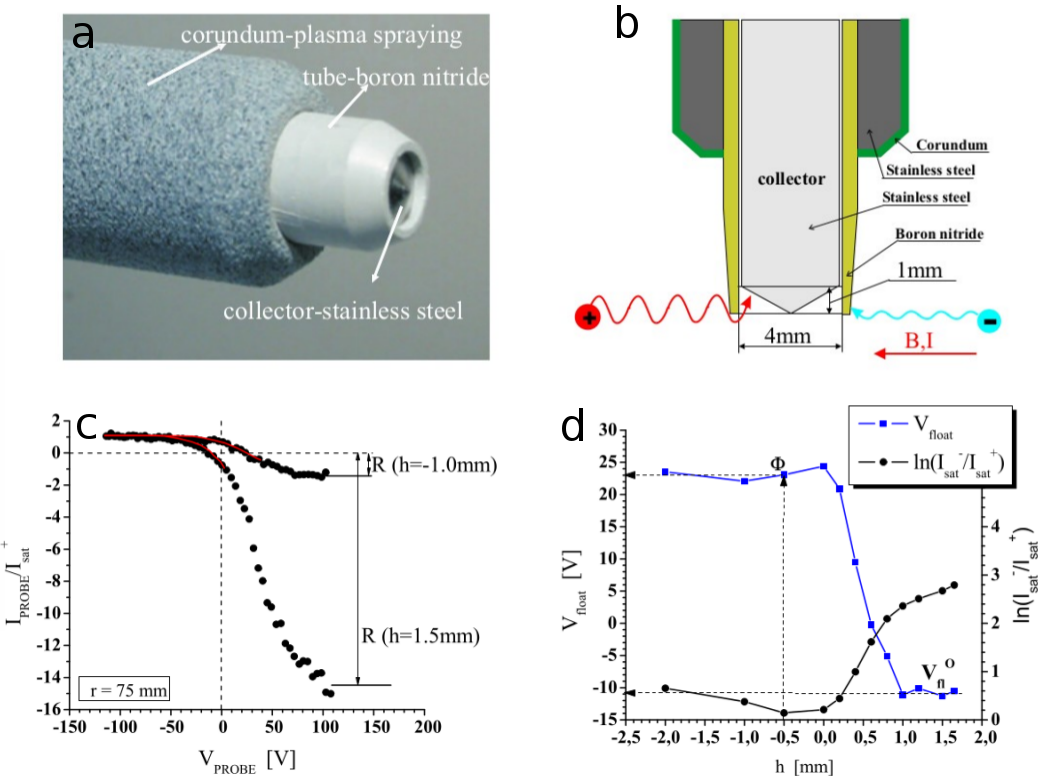
\includegraphics[height=15cm, width = 15cm]{adamek_orig_results}
\caption{Top: The orginal BPP designs by Adamek. Bottom: Measurements made by the BPP on the CASTOR tokamak. Figure c shows two I-V traces for the probe collector at different recession heights. Figure d displays the floating potential and the measured value of $\alpha_{BPP}$ for the collector as a function of recession height. Images taken from \cite{BPP} } %The BPP on MAST had a fixed retraction depth of 5 mm and a diameter of 4 mm }
\label{fig:adamek}
\end{figure}

Clearly there is strong empirical evidence for the success of the BPP technique however there are discrepancies between the experimental observations and the ideal theory. Firstly, $\alpha_{BPP}$ tends to zero but does not reach it, meaning there is always a higher electron saturation current to the probe than ion saturation current, even when the collector is recessed beyond multiple $\rho_i$. Ideal theory predicts negative values for $\alpha$ with sufficient probe recession as $I_e \to 0$ but this is not observed in experiments. These observations imply that the simple model, based on geometrical shadowing, is incomplete and significant transport perpendicular to the magnetic field must occur for electrons to still reach the collector surface once it is recessed beyond $\rho_e$.  Experiments with a flat BPP collector \cite{BPP_flat}, observed both ion and electron currents to the collector even when it was recessed beyond the ion Larmor radius, providing further evidence that cross-field transport must play a role in particle collection for the BPP. As such, a model for particle transport to the collector is required to verify the experimental results.

2D PIC simulations of the BPP have been carried out by Komm \cite{BPP-PIC}. In these simulations, the extent of the probe tunnel along the field was simulated as was the depth of the probe tunnel down to the collector but the direction perpendicular to the magnetic field was neglected for ease of computation so that the tunnel essentially had infinite width in this direction. These simulations verified the suitability of equation \ref{eq:ideal} for the BPP. However values of $\alpha_{BPP} <0$ were reported which have not been observed experimentally. This is in agreement with observations made from early 2D simulations carried out in VSim. It was found that when the direction perpendicular to the field was ignored, electrons could not reach the collector if it was recessed too far, suggesting that electric fields in the perpendicular direction were key to electron transport. If instead, both perpendicular directions were simulated, whilst neglecting the parallel direction, both ions and electrons were observed to reach the probe. This model does not accurately represent reality, as the probe tunnel now has infinite width parallel to the field, giving ions and electrons unlimited time to travel down the tunnel, perpendicular to the field, without coming into contact with a tunnel wall. Only 3D PIC simulations can fully capture the physics of the BPP.

 Detailed 3D PIC modelling of the ion sensitive probe (ISP) has been carried out by Komm \cite{komm-ION}. The probe is of a similar design to the BPP but both the   tunnel and collector are conducting and so can be biased to a potential independent of each other. It was found that a positive space charge region exists at the tunnel entrance as ions can penetrate deeper into the tunnel due to their large gyro-orbit. This leads to an electric field across the tunnel entrance and subsequently an E x B drift is established that drives electrons and ions downwards into the tunnel. The reported transport mechanism is supported by experimental work carried out by Sullivan \cite{sullivan2013internal}, in which an ISP was designed with a circular collector split into two semi-circles. This allowed the current collected by each half of the collector to be analysed independently. During electron collection mode, where the collector was biased positively with respect to the tunnel walls, an asymmetry in the electron current collected by each half was observed. This asymmetry was consistent with the direction of the E x B motion expected, due to the electric field created by the collector and wall potentials. It is believed that a similar mechanism is also responsible for transport of electrons into the BPP tunnel but 3D PIC simulations are required to confirm this. This chapter continues by detailing the 3D particle-in-cell simulations of the BPP, with a flat collector, carried out in order to explore the transport mechanism that allows electrons and ions to be collected. Simulations demonstrate the capability of perfect diagnostics within the constraints of Monte-Carlo noise. The plasma potential is known at each grid point and as the velocity of each particle is tracked, the electron temperature is also known. The simulations can therefore assess how well the BPP can reproduce input parameters of the simulation.% determine if the BPP truly measures the plasma potential.



 
\section{The Simulation Model} \label{section:model}
The simulation model is fully three dimensional (3D3V). The simulation domain captures a region of the probe head, the entire BPP tunnel down to the collector and a region of plasma above the probe at least four ion gyro-radii in depth in order to capture the magnetic presheath (MPS). The simulation domain is a cubic 3D Cartesian grid. The collector lies in the y-z plane at the bottom of the probe tunnel as illustrated in figure \ref{fig:bpp_both_views}.  At the beginning of the simulation, the plasma region is filled with a quasi-neutral plasma, with velocities sampled from a Maxwellian distribution. The motion of individual particles is tracked as they move due to self-consistent electric fields and an imposed uniform magnetic field. Particles that hit the probe structure deposit their charge to that location and are then deleted from the system. A charge density and electrostatic potential evolve naturally, to a steady state without imposing additional boundary conditions on the walls.  Particles are injected along the top plane of the simulation at $x=0$ to replenish those lost to the probe. The component of the velocity parallel to the magnetic field is sampled from the Emmert distribution \cite{Emmert}. The two perpendicular components are sampled from Maxwellian distributions.  The y and z axis are periodic and the magnetic field makes an angle $\theta$ with the y-axis. The plasma potential is fixed at the top of the simulation to be 0 V. 

The plasma density and temperature, modelled in the simulations was restricted by computational demands. Typical simulated parameters are shown in table \ref{tab:sim_parameters}. These values are close to those found in the SOL of MAST \cite{MAST_SOL}, however the simulated density is an order of magnitude lower than in experiments. Each grid cell in the PIC simulation was half a Debye length to prevent non-physical plasma heating in the simulations \cite{bible}. Increasing the density reduces the required grid spacing and so more grid cells are needed to simulate the same spatial region. To determine the effect of density, a selection of comparison simulations were carried out with an increased density of $n = 1.0 \, \times \, 10^{18} \, m^{-3}$ which is more in line with MAST's conditions. The increased density had no significant effect on the simulation results and so lower density simulations were run to produce the following results.
\begin{table}[]
	\centering

	\begin{tabular}{c|c|c}  %{lllll}
		 &  &  \\ % \\ \hline 
		Magnetic field strength $B$             & 0.54 T                                               \\
		Magnetic field inclination $\theta$                & $10^{\circ} $      \\
		Plasma density $n$               & $6.5 \, \times \, 10^{17} \, m^{-3}$ \\ 
		Electron temperature $T_e$ &      $ 60$ eV     \\ 
		Ion temperature  $T_i$ &     $60$ eV  \\  
		Ion Larmor radius $\rho_i$  &  $1$ mm  \\
		Electron Mass $m_e$ &  $9.11 \times \, 10^{-31}$ kg \\
		Ion Mass $m_i$ &  $900 \hspace{1mm} m_e$ \\
		Ion Charge $Z$ & $1.6 \times \, 10^{-19}$ C \\
	\end{tabular} 
		\caption{Typical plasma parameters used in the simulations of the BPP. }
		\label{tab:sim_parameters}
\end{table}


 
 
\begin{figure}[H]
\centering
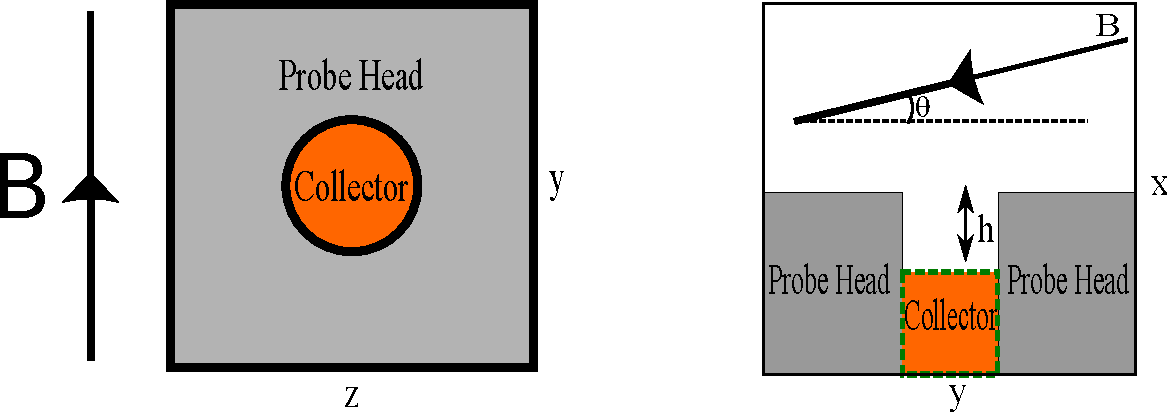
\includegraphics[width=0.9\textwidth]{figure1.pdf}
\caption{On the left - The BPP simulation domain as viewed from above looking along the x-axis. The collector sits at the bottom of the tunnel. On the right - A cross-section of the domain. $h$ is the recession depth. }
\label{fig:bpp_both_views}
\end{figure}


In experiments, the BPP is aligned with respect to the magnetic field such that the axis of the probe tunnel is perpendicular to the field. In our simulations, an angle $\theta$ was introduced as this was necessary for the particle injection algorithm. In order to inject particles, a source function must be specified in which to sample the newly injected particles velocity from. The rate of injection for both species must be specified too. In this model, particles are injected at the top of the domain to represent particles streaming along field lines from the bulk plasma. In the case of perpendicular alignment ($\theta$ $={0} ^{\circ}$), particle injection from the top of the domain would represent particles that have entered the domain due to cross-field transport mechanisms. A Maxwellian velocity distribution for these particles may be a valid assumption but the rate at which ions and electrons would enter the domain due to cross-field transport is not known. An alternative model was tested in which particles were injected along the y-axis, however, injecting particles on a periodic boundary led to the creation of artificial electric fields in the domain and so work proceeded with the original model. The results discussed below are for a field alignment value of $\theta$ $={10} ^{\circ}$. Additional simulations were carried out with $\theta$ ranging from  ${5} ^{\circ} \to {15} ^{\circ}$. Varying $\theta$ had no significant effect on the simulation results, but the  ${5} ^{\circ}$ case required more time to reach a steady state, as the ions take a longer time to propagate along the simulation domain for smaller angles. $\theta$ $={10} ^{\circ}$ was chosen as a compromise between shorter run times and matching the experimental set-up. This was the value used by Komm in simulations of the ISP \cite{komm-ION}.
A crude attempt at particle injection for the case of a perpendicular field was made in which particles were re-injected into the top of the simulation domain, with a Maxwellian velocity distribution, at the rate at which they were lost to the absorbing surfaces in the simulation. In this set-up it was found that the top surface of the probe-head floated positively with respect to the plasma potential as the ions were the more mobile species due to their large Larmor orbit. As discussed in Chapter 2.X,  this observation was expected as $\theta < \theta_c =  {\left(\frac{m_e}{m_i}\right)}^{\frac{1}{2}}$ \cite{stangeby-angles}. In an experiment, the alignment of the probe will never be perfectly perpendicular to the magnetic field. A misalignment above the critical angle, $\approx {1} ^{\circ}$ for deuterium, will allow electrons to stream along field lines to the surface, causing that surface to float negatively with respect to the plasma potential.


Collisions between charged particles are neglected in these simulations. The mean-free path ($\lambda$) for both electrons and ions significantly exceeds the length of the simulation domain ($\approx 5$ mm) for the plasma parameters used. From  \cite{Wesson}, using the stated simulated plasma parameters in table \ref{tab:sim_parameters}, $\lambda_{electron} = 7.2$ cm and $\lambda_{ion} = 10$ cm.  As a result, particles can travel across the simulation domain multiple times without experiencing a collision. The simulation plasma consists of electrons and singly charged ions with no neutrals or impurities present. Plasma-surface interaction effects such as secondary electron emission and sputtering have also been neglected.



\section{Transport Mechanism}  \label{section:transport}
Electrons and ions are observed to reach the collector in both experiments \cite{BPP} and the simulations even for collector recession depths beyond $2$ $\rho_i$. This observation implies that a cross-field transport mechanism is present driving particles down the tunnel. In the bulk plasma, particles are born at the top of the domain and travel along field lines towards the probe where they will either encounter the top surface of the probe head or will enter the tunnel. From the viewpoint of an observer looking along  magnetic field lines, the electron's clockwise orbit takes them towards the left hand side of the tunnel, whilst the anti-clockwise orbit of the ions takes them deep into the right hand side. This is demonstrated in figure \ref{fig:orbits}.
\begin{figure}
	\begin{center}
		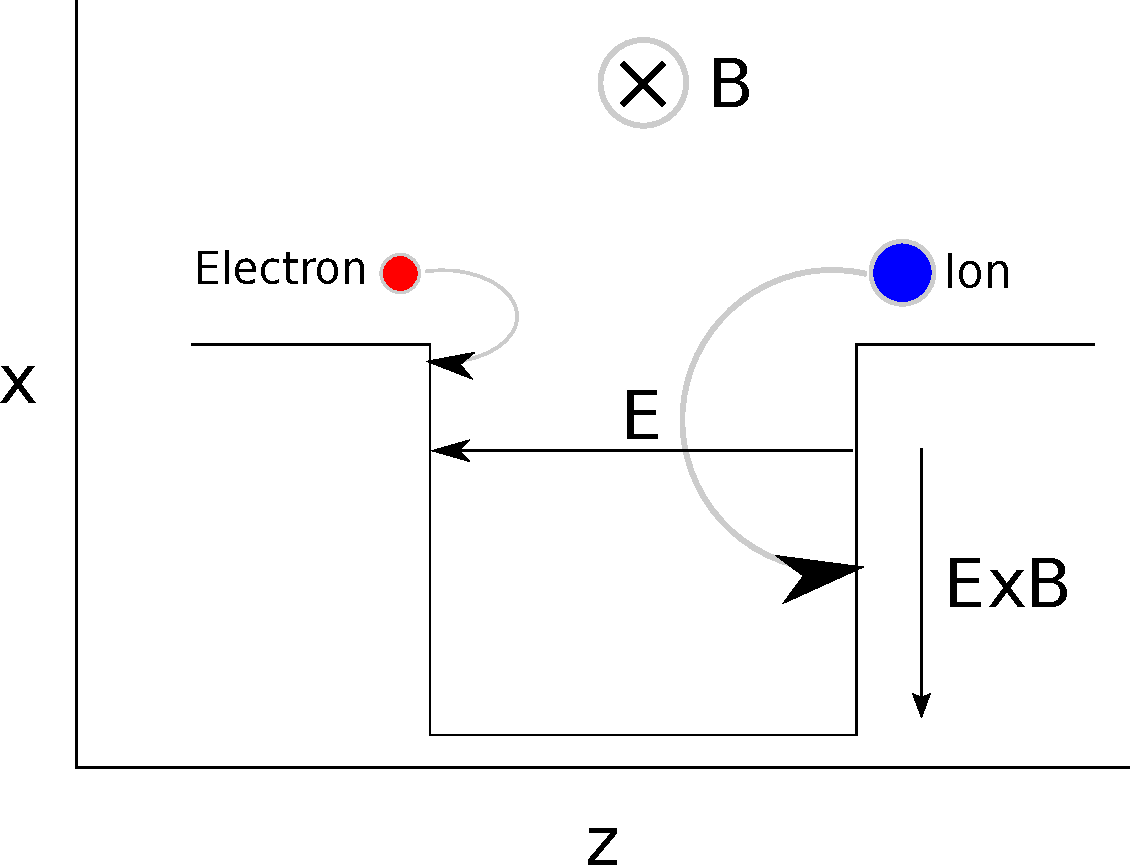
\includegraphics[width=.45\textwidth]{orbits.pdf}
		\caption{Electrons and ions orbit in opposite directions. Orbit of the ions takes them deep into the right hand side of the probe.}
		\label{fig:orbits}
	\end{center}
\end{figure}
This results in an electric field across the tunnel of the probe in the negative z direction. The potential structure within the probe tunnel and the resulting electric field is shown in figure \ref{fig:phi_plots}. 
\begin{figure}[H]
	\setbox0\hbox{%
		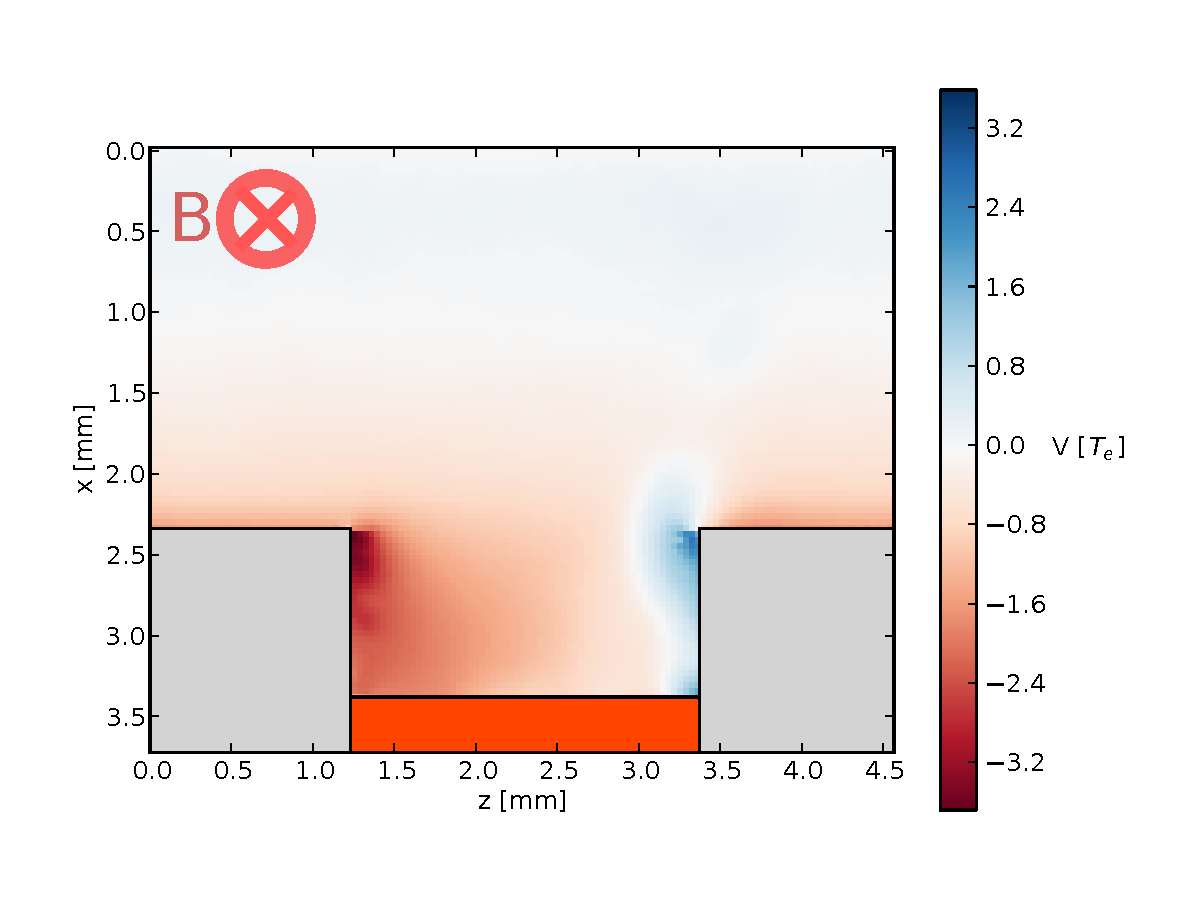
\includegraphics[width=.5\textwidth]{figure2.pdf}%
	}%
	\setbox2\hbox{%
		%\includegraphics[width=.5\textwidth]{top_down.pdf}%
		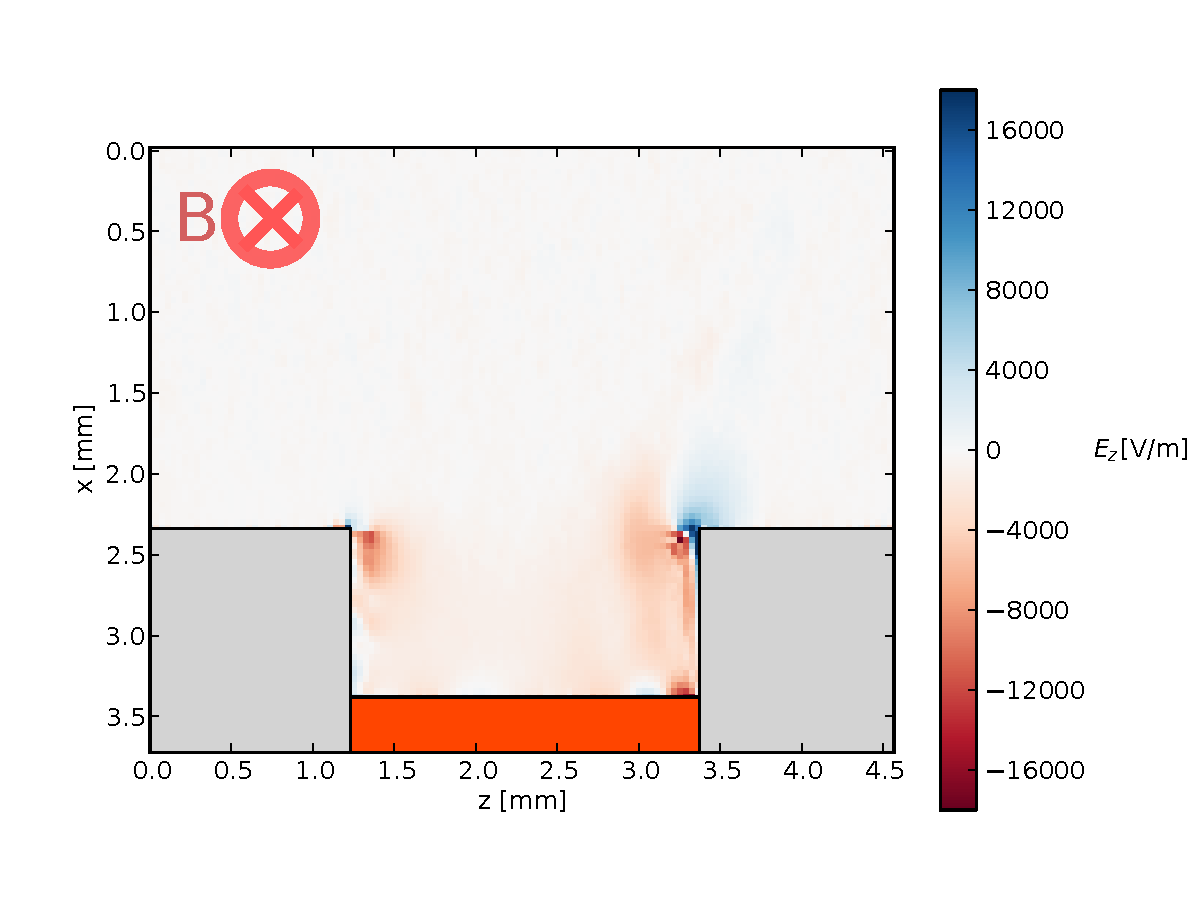
\includegraphics[width=.5\textwidth]{figure3.pdf}%
	}%
	
	\noindent
	\parbox{.5\textwidth}{%
		\centering
		\unhbox0
		
	}%
	\hfil
	\parbox{.5\textwidth}{%
		\centering
		\unhbox2
		
	}%
	
	\caption{On the left - cross section of the electric potential.  On the right - cross section of the resulting electric field in the z direction. Recession depth, $h = 1.1$ mm. Particles follow the magnetic field lines into and out of the plane shown. Their orbits can take them into contact with the walls, running parallel to the magnetic field, resulting in the potential structure shown.}
	\label{fig:phi_plots}
\end{figure}
The interaction between the electric field in the z direction and magnetic field in the y direction results in an E x B drift that drives particles down the x-axis to the collector (for directions of coordinate axes the reader is referred to figure \ref{fig:bpp_both_views}). Although the driving mechanism for the cross-field transport is the same for both species, their trajectories down the tunnel are very different. Once in the tunnel, particles will still continue to travel parallel to the field lines (along the y-axis) towards the tunnel wall. If a particle comes into contact with the tunnel wall it deposits it's charge there and is lost from the simulation. In terms of motion parallel to the field, electrons are the more mobile species due to their low mass.  As a result, a sheath forms in front of the floating tunnel wall to retard the flow of electrons. Only the most energetic electrons overcome this sheath potential to reach the wall. The less energetic electrons will reflect off the sheath and travel towards the other side of the tunnel. At the same time the electrons are driven down the tunnel due to the E x B drift. As a result, the electrons follow an oscillatory path down the tunnel. The trajectory of an electron, taken from the simulation, that reaches the collector is shown in figure \ref{fig:traj_e}. 
\begin{figure}[H]
	\begin{center}
		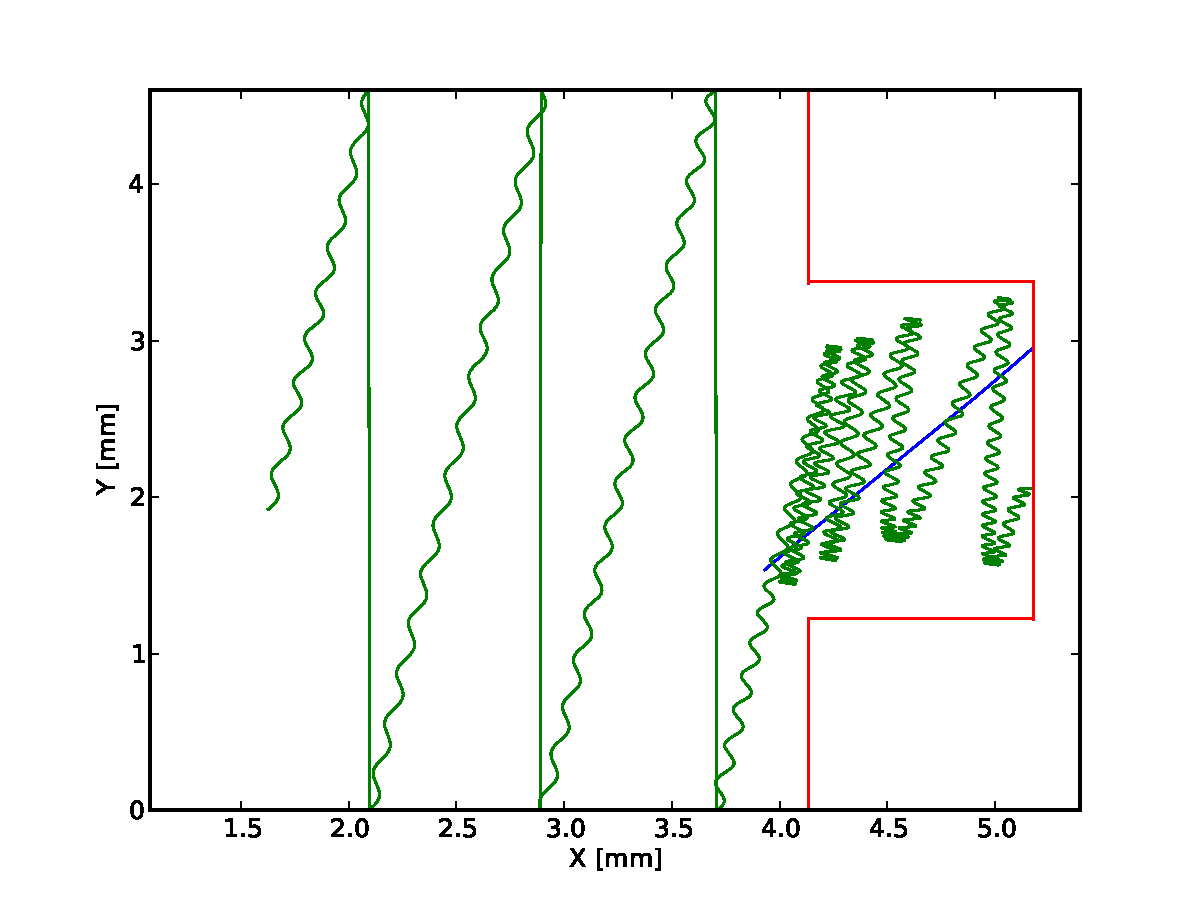
\includegraphics[width=.75\textwidth]{figure4.pdf}
		\caption{The trajectory of electrons and ions in the x-y plane is shown in green and blue respectively. Red lines show the walls of the probe. The electron follows the field across the periodic simulation domain until it enters the tunnel. Once in the tunnel the electron reflects back and forth due to the sheath potential. Vertical lines represent the electron leaving the simulation on one side of the periodic boundary and re-emerging on the other side. Ions simply travel down the tunnel due to their orbit whilst travelling parallel to the field.   $h = 1.1$ mm.  }
		\label{fig:traj_e}
	\end{center}
\end{figure}
The most energetic electrons are lost at the top of the tunnel as they are able to overcome the sheath potential. Therefore a less negative potential is required to maintain floating conditions further down the tunnel. The sheath potential on the wall becomes less negative with depth varying from -200 V at the top of the tunnel to -140 V at the bottom. 
As a result more and more of the electron population is lost to the walls with only the least energetic not capable of overcoming progressively weaker sheath potentials to make it to the bottom of the probe. The parallel velocity distribution of electrons at the top and bottom of the tunnel is shown in figure \ref{fig:hists}. The width of the distribution narrows deeper into the tunnel as the high energy electrons are lost to the wall.

\begin{figure}[H]
	\begin{center}
		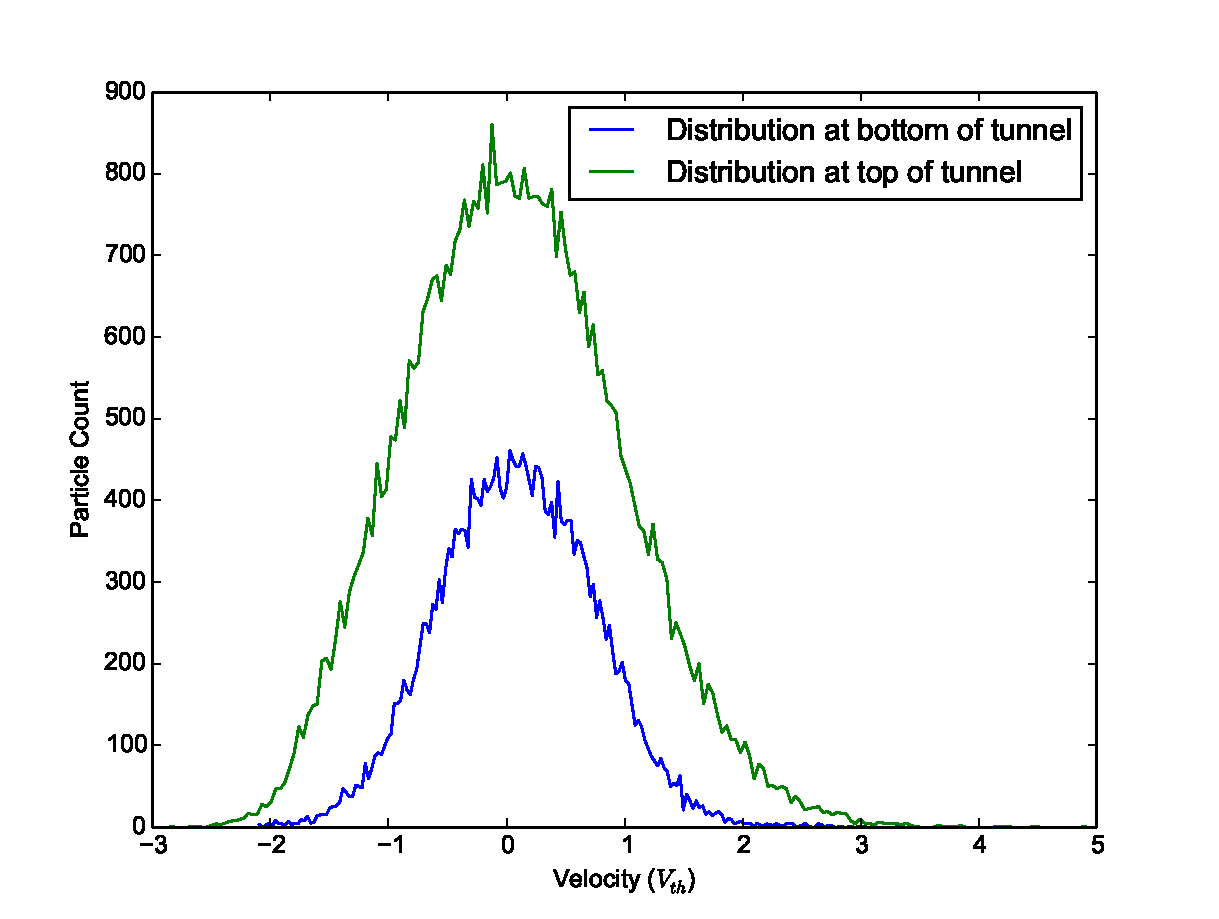
\includegraphics[width=.75\textwidth]{electron_hists.pdf}
		\caption{The parallel velocity distribution for electrons at the top and bottom ($h = 1.1$ mm) of the BPP tunnel. The distribution narrows deep into the probe as the more energetic electrons are able to overcome the sheath potential and hit the wall. }
		\label{fig:hists}
	\end{center}
\end{figure}



The tunnel sheath acts to accelerate ions towards the wall so any ions that enter the sheath will be lost to the walls and unable to make it to the probe collector. Once entering the tunnel, an ion will continue its Larmor orbit whilst travelling parallel to the magnetic field towards the wall. To be collected  an ion must have sufficient perpendicular velocity to make it to the probe before it's parallel velocity takes it to the wall i.e. 
\begin{equation}
\left(\frac{h}{v_\perp} \right) < \left(\frac{d}{v_\parallel} \right)
\end{equation}
where $h$ is the recession depth of the probe and $d$ the tunnel diameter. Ions that reach the probe collector have a higher perpendicular energy than parallel energy when they enter the tunnel. Their perpendicular speed is increased in the tunnel due to the E x B drift. The Larmor radius of the ion must also be sufficiently large so that the ion can reach the collector, i.e.
\begin{equation}
\rho_i \geq h
\end{equation}



The contrast in the collection mechanism for ions and electrons was predicted in \cite{BPP-MAST}. The collection mechanism suggests that the proportion of the electron population that can make it to the collector should not be sensitive to the probe tunnel diameter. The electron parallel velocity will always exceed the E x B drift velocity so electrons will encounter the wall sheath multiple times before they are able to drift to the collector. On the other hand, the collection of ions should be sensitive to the probe diameter. If the probe is too narrow, ions will not have time to complete enough of their orbit to make it to the collector before encountering the tunnel wall. The tunnel must be sufficiently wide so as not to hinder the collection of the ions. This is investigated in section \ref{Diameter}. 


\section{Does the Probe Measure the Plasma Potential?} \label{Plasma_Potential}
In order to test the capability of the BPP to measure the plasma potential, simulations were carried out for a probe of diameter 3.2 mm and a depth of 1.04 mm. A simulation was carried out with the probe operating in floating mode to obtain a floating potential measurement ($V_{BPP}$). Further simulations were carried out in order to determine $R$ and $\alpha_{BPP}$. In these simulations, the probe was biased positively and negatively with respect to the plasma potential in order to determine  $I^-_{sat}$ and $I^+_{sat}$ respectively. It was observed that the currents for both species did not saturate. This behaviour has also been observed in experiments \cite{adamekfast}. Following the method of \cite{adamekfast}, it was necessary to carry out further simulations with different probe bias voltages. The currents obtained at each voltage could then be extrapolated to obtain the value of $R$ at the plasma potential. 


  
The saturation currents increase linearly with probe bias, therefore it was possible to estimate $R$ by linearly interpolating both currents to the plasma potential and defining their saturation values to be at this point. The values for the currents give $R =3.02$ corresponding to a value $\alpha_{BPP}= 1.1$. These values are higher than what is typically observed in experiments where $\alpha_{BPP}$ is in the range 
\begin{equation}
\alpha_{BPP} = 0.6 \pm 0.3 
\label{eq:accepted_range}
\end{equation}
However, these estimates were obtained using probes of at least $4$ mm in diameter. In section \ref{Diameter}, it is shown that a larger probe size reduces $R$ closer to the value measured in experiments. Nevertheless, if it can be demonstrated that the BPP floats at a potential offset from the plasma potential by the product of $T_e \alpha_{BPP}$ then the BPP mechanism will be validated. Shown in figure \ref{fig:potential_profile} is a plot of the potential across the simulation domain along the x-axis. The potential at each point represents the average potential across a circular cross-section centered over the BPP collector. The plasma potential is defined as the value at the top of the domain, where the profile is flat before the magnetic presheath (MPS) potential drop. The probe is found to float at a potential of $-69$ V relative to plasma potential. Based on the values of $\alpha_{BPP}$ and $T_e = 60$ eV,  equation \ref{eq:ideal} predicts the plasma potential should be $-3.8$ V.  This is very close to the value for the plasma potential in the simulation (0 V). The BPP will therefore float at a potential offset from the plasma potential by a factor of $T_e \alpha_{BPP}$. An $\alpha_{BPP} = 0$ would be required for the BPP to truly float at the plasma potential.


\begin{figure}
	\begin{center}
		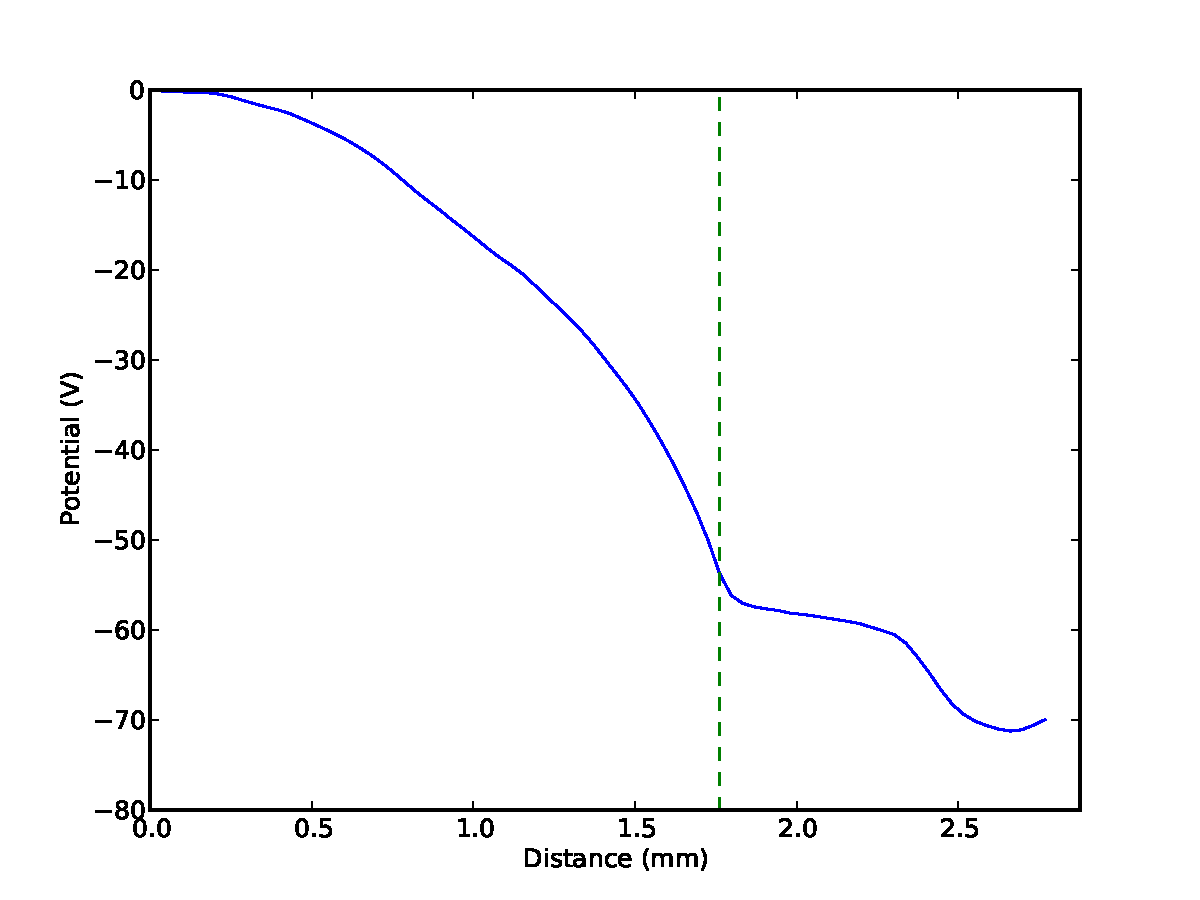
\includegraphics[width=.75\textwidth]{figure5.pdf}
		\caption{The plasma potential across the simulation domain, the dashed line shows the location of the BPP tunnel entrance. }
		\label{fig:potential_profile}
	\end{center}
\end{figure}


Simulations were carried out with an increased electron and ion temperature of 120 eV to determine if particle temperature had an impact on $\alpha_{BPP}$. As before, multiple simulations were carried out for different probe bias voltages so that $\alpha_{BPP}$ could be measured by interpolating the currents.  For these runs, a value of $\alpha_{BPP} = 1.38$ was observed, which is not significantly higher than the value found for $T_e$ = 60 eV  ($\alpha_{BPP} =1.1$). It does not appear that the temperature strongly effects the operation of the BPP over the range of $60 eV \leq T_e \leq 120eV$ considered in this study.



\section{Can the probe be used to make Electron Temperature measurements?} \label{section:temperature}
Additional simulations were carried out in order to test the capability of the BPP-LP pair to make electron temperature measurements. The BPP was replaced with a flush-mounted probe (FMP) and operated in floating mode to obtain $V_{LP}$. As discussed previously in section \ref{Plasma_Potential}, $\alpha_{BPP}$ and $V_{BPP}$ have already been measured. As in experiments, our simulations are not capable of measuring $\alpha_{LP}$. In magnetised plasma the collection length of the probe operating in electron collection mode can extend very far into the plasma. It is not possible to capture this region in our simulation domain and so it is not possible to collect $I^-_{sat}$. Following experimental procedure we will therefore use the theoretical value for $\alpha_{LP}$ provided by equation \ref{eq:Stangeby}.

As before, results are stated for the $3.2mm$ diameter probe with an electron temperature of $60eV$. The FMP is found to float at a potential $V_{LP} = -129$ V. Combining this with $\alpha_{BPP}= 1.1$, $V_{BPP} = -69 $ V and the theoretical value of $\alpha_{LP} = 2.14$ for the reduced ion mass we obtain a value of $T_e = 58.3$ eV which is in very good agreement with the specified temperature. This method is a viable way of making fast electron temperature measurements provided $\alpha_{BPP}$ is known. The measurement of $T_e$ can be combined with $V_{BPP}$ to determine the plasma potential.


\section{Ball-Pen Probe Design Considerations} \label{Design}
\subsection{Effects of Probe Diameter} \label{Diameter} 
In order to investigate the effects of probe diameter, three probes of different width were simulated. The probe diameters were a)  1.08 mm,  b) 2.16 mm and c) 3.24 mm. All probes were recessed to the same depth of 1.04 mm. The ion Larmor radius in the simulations was $\rho_i =1.02$ mm. For each probe diameter, three simulations  were carried out: one with the probe operating in floating mode and two biased cases where the collector was in ion collection and electron collection mode. The floating potential of the collectors is shown in figure \ref{fig:float_diam} along with the measured value of R. The ratios presented were obtained by dividing one current for each species. A linear interpolation has not been carried out so the true value of R is not known. The values are presented here as they demonstrate the effects of probe diameter on BPP measurements even if their absolute value is not correct. 

\begin{figure}[H]
	\begin{center}
		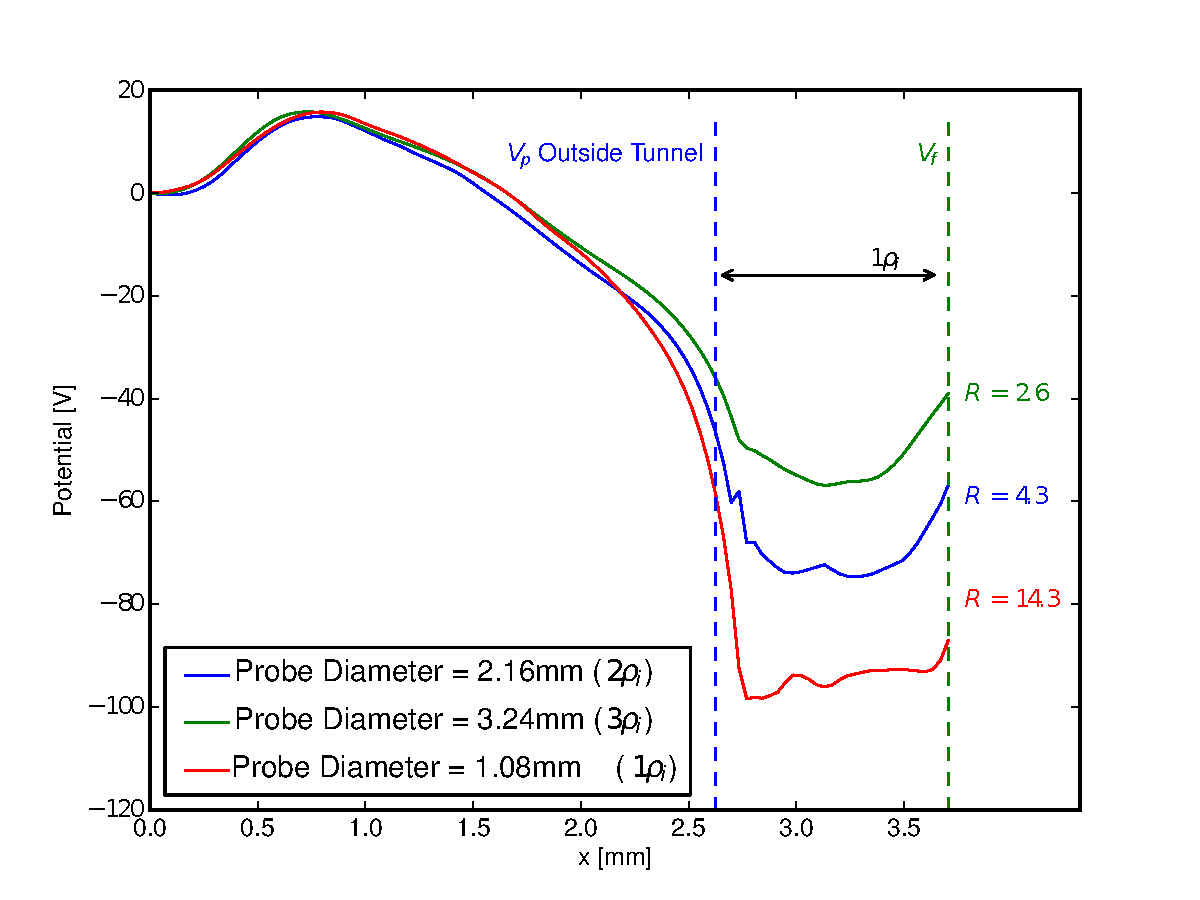
\includegraphics[width=.75\textwidth]{figure6.pdf}
		\caption{The potential structure across the simulation domain. The floating potential of the probe varies with tunnel diameter as does the value of R. The potential structure near $x=0$ is a result of the source sheath, an artefact of particle injection in this region. }
		\label{fig:float_diam}
	\end{center}
\end{figure}

With increasing width, a lower ratio R and a less negative value for $V_{BPP}$ is observed. Beginning with the ions we find the current per unit area increases as the diameter increases. This is consistent with the collection mechanism: with a wider probe, ions have more time to reach the probe before their parallel motion brings them to a tunnel wall, therefore a higher proportion of the ion population reaches the probe. The electron current per unit area remains approximately constant with increasing probe diameter. 




In order to allow a direct comparison with experiments, a set of simulations with a probe diameter of 4 mm and depth of 1 mm were carried out using a realistic ion mass and a field strength of 1.3 T, equivalent to the conditions used by Ad{\'a}mek et al in \cite{BPP}. The following measurements were obtained
\begin{equation}
R = 2.8 \>\>\>\>   \alpha_{BPP} = 1.04 \>\>\>\>   V_{BPP} = -67.6 \space V 
\end{equation}
which are in good agreement with equation \ref{eq:ideal}. However, the value for $\alpha_{BPP}$ obtained in the simulations is outside the accepted range derived from experiments given in equation \ref{eq:accepted_range}. This range is obtained using conical collectors where as the simulated probe was flat. The effects of BPP diameter were investigated on the linear plasma device Mirabelle \cite{mirabelle}. However, due to the low magnetic field strength used in the experiments, the electron Larmor radius was comparable to the tunnel diameter and the effectiveness of the probe to shield the electron current strongly depended upon the probe geometry. This regime of operation is not applicable to the simulations carried out. To the authors knowledge, an experimental comparison of the influence of probe diameter on the value $R$, for fusion relevant plasmas,  has not been reported.  However, in \cite{bpp_diameter}, three BPPs with a flat collector were placed into the edge region of CASTOR together with a BPP with a conical collector to make simultaneous measurements of the plasma potential. The flat collector probes were of different diameter: 1 mm, 2 mm and 4 mm and the conical collector had a diameter of 2 mm. The authors concluded that the diameter was not a critical construction parameter but differences in the value of the measured plasma potential were observed. Values for $R$ were not reported. Differences in the plasma potential measurements were attributed to a misalignment of the probes with the magnetic field. However, in the region of minimal curvature of the poloidal field, where the misalignment was lowest, it was found that the floating potential of the flat collector probes increased with probe diameter. If the floating potential of the probe varied with probe diameter, this could indicate that the value of $R$ also changes with probe diameter. Out of the four probes, the 2 mm conical BPP was consistently found to float at the highest potential. This would suggest a smaller diameter conical BPP can achieve the same ratio $R$ as a larger, flat collector BPP. The differences in potential measured in experiment were not as extreme as the differences found in the simulations. However, in the simulations, $T_e$ = 60 eV compared with $T_e$ = 20 eV in this experiment. This does not effect the capability of either probe to make plasma potential or electron temperature measurements, provided $\alpha_{BPP}$ is known for the probe that is employed. 

\subsection{Effect of Probe Recession}
In the experiment described in \cite{BPP} it was found that the value of R reached a minimum when the probe was recessed 0.5 mm ($1\rho_i$). Once the probe was recessed beyond this depth, the value of R increased. Simulations have been carried out to test the sensitivity of R on collector recession and have found a similar trend. Both electron and ion currents to the probe decrease as the probe is recessed deeper into the tunnel, as more particles are absorbed by the tunnel walls. However, the electron current decreases less strongly than the ion current as electrons can reflect off the sheath formed along the interior walls of the probe while being driven towards the collector by E x B drifts. The reduced electron current is a result of the potential on the tunnel wall decreasing with depth into the tunnel, i.e. it becomes closer to the plasma potential. As a result, less of the electron population will be reflected by the weaker sheath potential. Increasing the probe depth makes it more likely that an ion's parallel velocity will take it into a tunnel wall before it can make it down to the collector. It appears that as long as the BPP is recessed beyond a few $\rho_e$ the electrons become magnetically shielded and can only access the collector with E x B drifts. The probe then operates as a BPP. As long as this criteria is met and the probe depth is fixed with known $\alpha_{BPP}$  the probe depth is not thought to be an important parameter. However, beyond a certain depth, most ions will be absorbed before making it to the collector and the measurements will become dominated by noise. Simulations and experiments suggest a depth of 1 mm is sufficient for tokamak plasma conditions in order to minimise $\alpha_{BPP}$.   
 




\section{Conclusions and Future Work}
3D3V PIC simulations have verified that the BPP measures a potential offset from the plasma potential by a factor $T_e \alpha_{BPP}$. BPPs in practice have obtained values as low as $\alpha_{BPP} =0.6$. For electron temperatures on the order of $10$ eV, the difference between the floating potential of the BPP and the plasma potential will then be several volts.  The floating potential measurement from the BPP is closer to the plasma potential than the floating potential of a standard Langmuir probe, however, the electron temperature is still required to determine the plasma potential from the BPP floating potential measurement and so the BPP is not capable of providing direct measurements of this quantity. By simulating both a LP and a BPP the source temperature for the electrons was recovered, validating the BPP-LP method for making fast electron temperature measurements. Using a BPP and LP, operated in floating mode, in close proximity to each other could then provide fast measurements of $T_e$ which can then be used to determine $\Phi$.

The mechanism that allows electrons to reach the collector even when it is recessed far beyond their Larmor radius has been confirmed. Inside the tunnel, electrons oscillate along field lines, reflected by the wall sheaths, whilst simultaneously undergoing E x B drift motion towards the collector. The larger orbit of the ions allows them to reach deeper into the tunnel, their perpendicular motion further facilitated by the E x B drift. Ions must reach the collector before their parallel motion brings them to a tunnel wall. This mechanism suggests the probe diameter could be an important construction parameter. Further experimental measurements are needed to verify this. Larger $\alpha_{BPP}$ values are obtained in the simulations than in experiment. Possible reasons for this discrepancy are that a flat collector was simulated, experimental $\alpha_{BPP}$ values have only been reported for conical collectors, conical collectors may reduce the ratio $R$ more efficiently. The simulation that was completed with realistic ion mass, in order to directly compare against Adamek's original measurements, simulated electrons and ions at a temperature of $60$ eV, whereas in the experiment, the temperature was estimated to be $10$ eV. Reducing the simulated temperature would have increased the number of grid cells to be simulated, making the simulations too computationally expensive. Based on the $120$ eV simulations carried out, it is not thought that the temperature would have a significant impact on the simulated $\alpha_{BPP}$. A final cause of the discrepancy could be the exclusion of secondary electron emission (SEE) from the BPP collector. SEE could occur when an ion strikes the surface of the collector, An electron emitted from the surface of the collector would be the same as an ion collected by the surface. SEE could then act to enhance the measured ion current, reducing the measured value of $\alpha_{BPP}$. It would be of interest to add a SEE model into the PIC simulations and test this effect on the BPP measurements.  




 Probe depth is not an important consideration, provided the collector is recessed sufficiently such that the electrons are magnetically shielded from the collector. It was found that recessing the probe a depth greater than several $\rho_e$ is sufficient. The voltage applied to a BPP should be swept initially in experiments to measure $\alpha_{BPP}$. Once this value is acquired it is then possible to use the BPP to extract the electron temperature and plasma potential.

The simulations in this chapter focused on fusion relevant plasma conditions. The simulations could be extended to low-temperature devices such as the magnetron to test the capabilities of the BPP in these plasmas.  Although the lower temperatures will reduce the Debye length, this is offset by lower densities, allowing the Debye length to be resolved. This extension is carried out in Chapter X.









%Relies on the assumption that Te = Ti
	
%Describe ISP ion sensitive probes, how they can be used, are they more useful?
	
	
%Our alpha values are higher than in experiment, i.e are electron current is too high relative to our ion current. However we don't take into account SEE. An electron given off by the collector due to an ion hitting it, would register as an ion hitting the probe, an emitted electron lost = a collected ion gained, in experiments this could boost the ion current, lowering the value of R. So simulations taking into account SEE are required.	
	
	
%Look at Sullivan paper, I did some work on exploring which areas of the probe are hit the most is this worth talking about. I do have alpha values saved	
	
%is BPP method invalidated for perfect alignment of field ? 
% The mechanism for the BPP was then invalidated as recessing the probe would only further inhibit the electrons forcing the probe to float even more positively. However,   	
\section{References}
\bibliography{references}
	
\end{document} 

